\chapter{Introduction}
% Survey of static hover, multirotor control and relevant topics}
% Transcribe Antonio Franchi's Talk

% (Dexterous Hexrotor)

\begin{figure}[H]
        \centering
        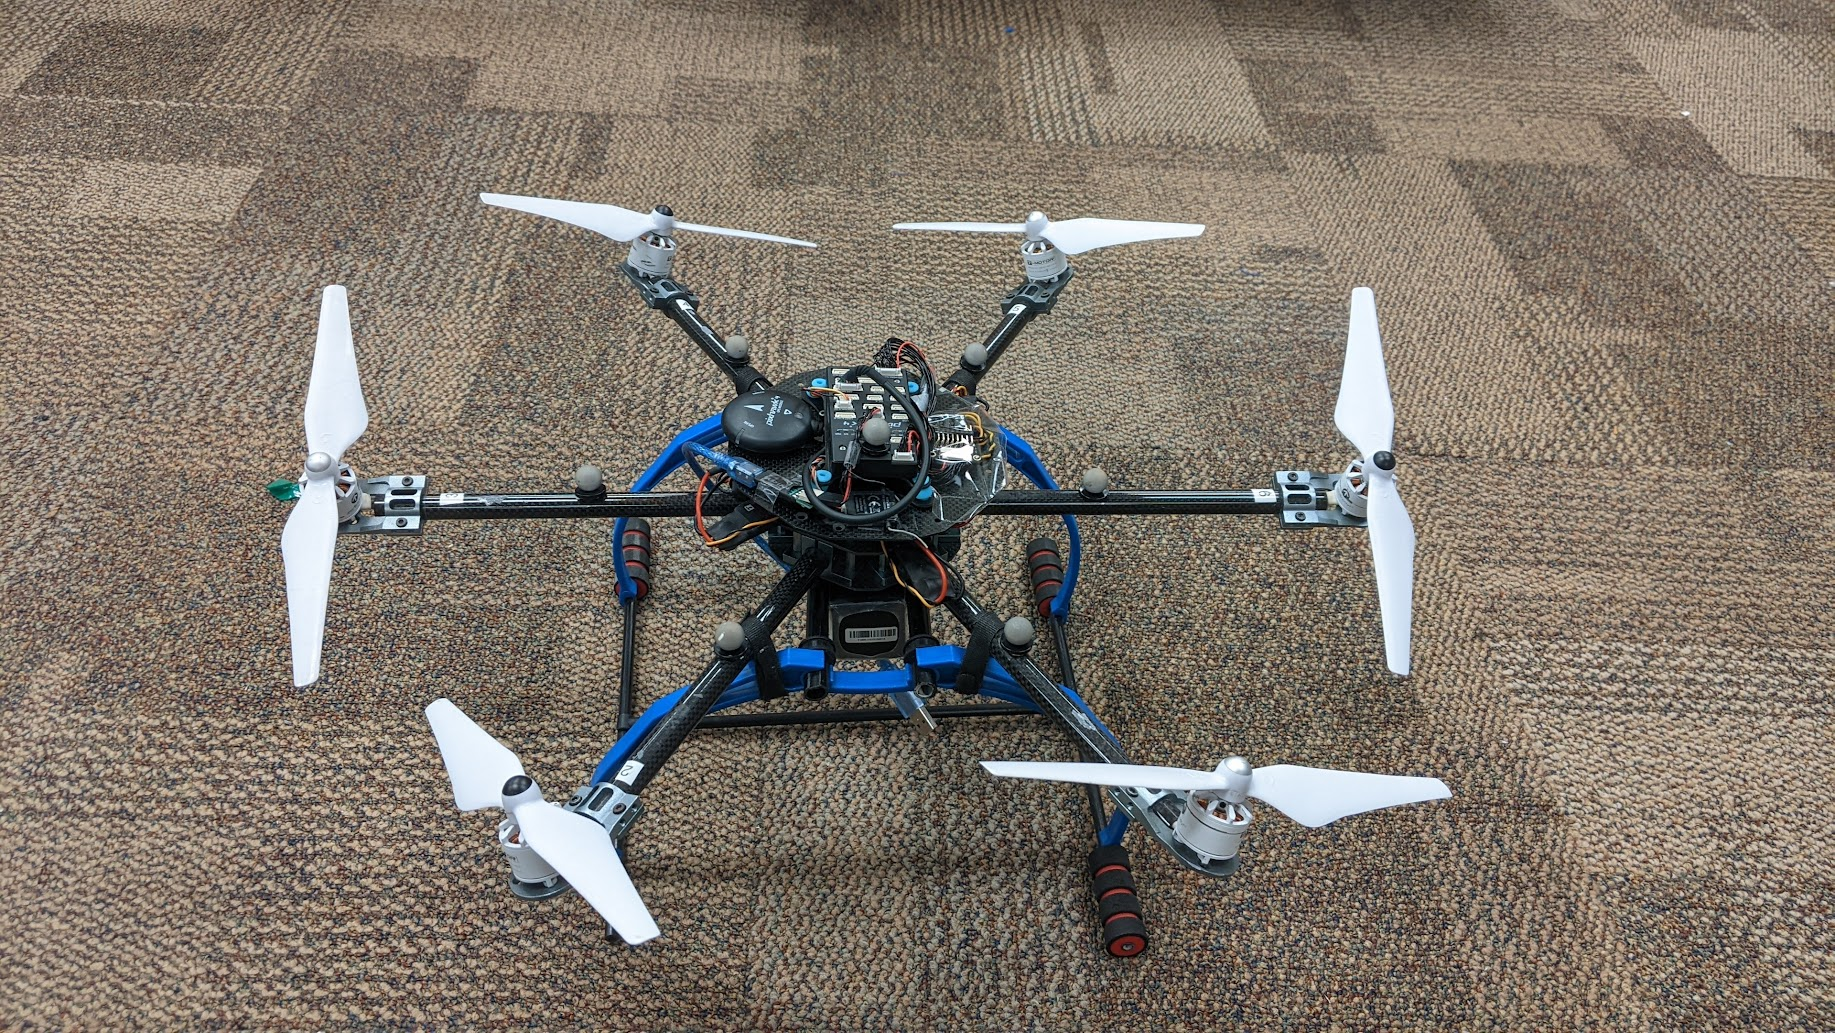
\includegraphics[width = 0.49\textwidth]{Part2/figs/drone.jpg}
        \caption{Tilted winged hexrotor (Dexterous Hexrotor)}
        \label{fig::drone}
\end{figure}


\par The fully actuated designs of unmanned aerial vehicles (UAVs) have gained a lot of prominence over recent years for
aerial manipulation (\cite{ding2021design}, \cite{ryll20176d}). Dexterous hexrotor (figure-\ref{fig::drone}) is one such
design with applications in physical interactions with structures (\cite{jiang2017estimation}). A notable design feature
includes tilted propellers allowing independent control over the six degrees of freedom in a limited region of the state
space. The rotational inertia and mass of the large propeller blades result in actuator dynamics with time-scales
comparable to that of the dynamics of the drone effecting the performance in application of precise and controllable
forces (\cite{hamandi2021design}). In fact, the survey of \cite{hamandi2021design} noted gaps in the literature coverage
regarding theoretical analysis of actuation limits for multi-rotor UAVs.

\par Several works propose actuator fault detection using the existing signals from the instrumentation such as
